\subsection{Page conditioning and line segmentation}
\label{sec:des-seg}
The recogniser needs one line of text at a time. A photographed page can contain shadows, rotation and strokes extending between lines. This stage prepares the page and returns ordered line crops while preserving the shape and spacing of the writing.

\subsubsection{Lighting normalisation and ink extraction}
Using a single global brightness threshold can mistake a shadow for ink if the page lighting differs. The design compares each pixel with its local background, following the local comparison used in adaptive thresholding, by calculating the background level for an area around each pixel~\cite[pp.~2--3]{bradley2007}. Image analysis uses a 0-255 grey image at half the resolution in each dimension by averaging $2\times2$ blocks. This is to ensure thin pixel lines get do not get missed. The full-resolution page is kept for the final crops.

\paragraph{Estimating the local background.}
The local background light level $B_r$ is the average light level of the background of a square window of radius $r$ around each grey pixel. The implemented radius is $r=\max(8,\min(40,\operatorname{round}(H/41)))$, where $H$ is image height. A summed-area table $S$, also call an integral image is a pre-calculated grid where each pixel stores the sum of all pixels up and to the left of it. It is used to calculate each window sum using four different image integral computations to isolate the window size in the middle.~\cite[p.~2]{bradley2007}.
\begin{equation}
\Sigma_{[y_0,y_1)\times[x_0,x_1)}=
S(y_1,x_1)-S(y_0,x_1)-S(y_1,x_0)+S(y_0,x_0).
\label{eq:des-integral}
\end{equation}

The window area divides the sum that was calculated to give $B_r$. Edge replication is done to avoid darkening or lightening the image boundary with artificial padding. This calculation is independent of window size once the pre-computed image integral is available.

\paragraph{Separating ink from paper.}
Dividing the grey intensity of each pixel $G$ by its local background calculation gives the ratio $R$. Ink has a lower ratio than paper. The binary mask $M$ retains pixels below threshold $T$, to effectively only store ink values according to a certain threshold, and exclude the background. The $y$ and $x$ in each case refers to the position of the pixel in the image.
\begin{equation}
R(y,x)=\frac{G(y,x)}{\max[B_r(y,x),1]},\qquad
M(y,x)=\mathbf{1}[R(y,x)<T].
\label{eq:des-ratio}
\end{equation}

The denominator floor avoids division by zero to prevent a maths error. Otsu's method is a technique which analyses the ratio values between the grey intensity of the pixel and the local background calculation, and finds the optimal dividing line to get the correct threshold. Otsu's criterion selects the threshold by maximising the separation between two histogram classes~\cite{otsu1979}. The class masses are $\omega_0,\omega_1$, with mean bin indices $\mu_0,\mu_1$.
\begin{equation}
T=\arg\max_t\ \omega_0(t)\omega_1(t)
\bigl[\mu_0(t)-\mu_1(t)\bigr]^2.
\label{eq:des-otsu}
\end{equation}

The software uses 256 bins to store the ratio values in a range of 0-1.2. Applying the threshold to a brightness ratio makes the decision less sensitive to gradual shadows than applying it directly to the grey image, hence the reason that local background calculation is used. SOURCE

This process was verified through a test example image from the dataset, to verify if an ink pixel was kept or rejected by the threshold. The pixel has an intensity of 100 and local background 161.43, giving $R=0.62$. Its selected threshold is 0.80, so the pixel is kept as ink. The prefix values and threshold calculation are retained in Appendix~\ref{app:worked-design-calculations}.

\subsubsection{Page orientation and skew correction}
A page that is rotated at $90^\circ$ has a completely incorrect axis line, meaning text segmentation could not occur, while a small rotation changes the slope of lines on that axis, and importantly still remains in the same line axis. To automatically know when to rotate a page, the software first compares the fraction of nearly empty rows before and after a $90^\circ$ rotation. A turn requires a score improvement by a factor of 1.35, which will avoid an unnecessary rotation when the evidence is weak and the facotr is not high enough.

Fine deskewing is a process that automatically straightens a document image with a small tilt until it becomes horizontal. It tests seventeen angles from $-4^\circ$ to $+4^\circ$ in $0.5^\circ$ steps. For each angle $p_\theta(y)$ is the projected count of how much row ink there is. When the ink is rotated and concentrated into its own fixed row, it increases the squared-profile objective~\cite{postl1986}.
\begin{equation}
\theta^*=\arg\max_\theta\sum_y p_\theta(y)^2,\qquad
p_\theta(y)=\sum_x M_\theta(y,x).
\label{eq:des-skew}
\end{equation}

The search will map the ink coordinates onto candidate rows in a further reduced mask. The selected rotation is then applied to the full and working grey images, and then the binary mask over the page dividing pixels between ink or background is rebuilt. The example test page in the appendix selects $+1.0^\circ$, with the trial scores retained in Appendix~\ref{app:worked-design-calculations}.

\subsubsection{Line detection and separation}
To properly separate a line, a line centres is used to locate the writing, while curved boundaries separate overlapping ascenders and descenders. A straight horizontal cut can split these strokes even when they belong to different lines, which is not ideal, hence the reason for the curved boundary cuts over ascenders and descenders.

\paragraph{Removing marks and locating line centres.}
A preliminary line pitch $P$ (the estimated spacing between text lines) sets the scale for filtering the surrounding background artifacts on a scanned page image, and printed rule lines (the straight horizontal lines going across the page). Horizontal and vertical run limits are 1.25 and 1.4 pitches. The pitch is estimated again after these marks and artifact components have been cleared out. A long handwritten underline can also meet a rule-removal condition if it remains within the specified pitch angles.

The final smoothed row profile is created and consists of candidate peaks above 6\% of its maximum. Median peak spacing gives the preferred pitch of the lines, with a lower bound based on component height. Autocorrelation and component height provide fallbacks. Centres are selected by peak strength (the max text height within its local range) with at least $0.6P$ separation.

\paragraph{Finding a boundary between lines.}
A boundary follows a low-cost path across each gap determined by the line centers and pitch. The local cost combines a strong penalty for crossing ink with a weaker attraction towards midpoint $y_m$, scaled by half-gap height $h_g$.
\begin{equation}
C(y,x)=4 M(y,x)
+0.012\left(\frac{y-y_m}{h_g}\right)^2.
\label{eq:des-seamcost}
\end{equation}

Here $M$ is the mask after morphological closing, which is a dilation operation (pixel expand) followed by erosion operation (pixel shrink), which is a method of expanding then shrinking pixel boundaries to bridge gaps or extend lines~\cite[p.~541]{haralick1987}. Closing with radius $\max(2,\lfloor0.07P\rfloor)$ fills narrow breaks that could otherwise let the boundary enter a stroke. The path is then computed dynamically using the accumulated cost $D$~\cite[p.~3]{avidan2007}. The equation that follows is a dynamic path-finding algorithm, used to track the the curves of the text.
\begin{equation}
D(y,x)=C(y,x)+\min
\{D(y+d,x-1)+0.02|d|\}.
\label{eq:des-seam}
\end{equation}
$C(x,y)$ refers to the local cost of passing through the pixel at x,y, and d refers to the vertical displacement and step size.

Figure~\ref{fig:des-seam-example} shows one gap from Abhinav01. It was selected for the largest reduction in crossed ink on that page. The seam crosses one working-image ink pixel, compared with 64 for the straight midpoint cut. The lower panel shows the cost field that makes the seam bend around the writing. The second example and complete original figure are in Appendix~\ref{app:extended-design-figures}.
\begin{figure}[H]\centering
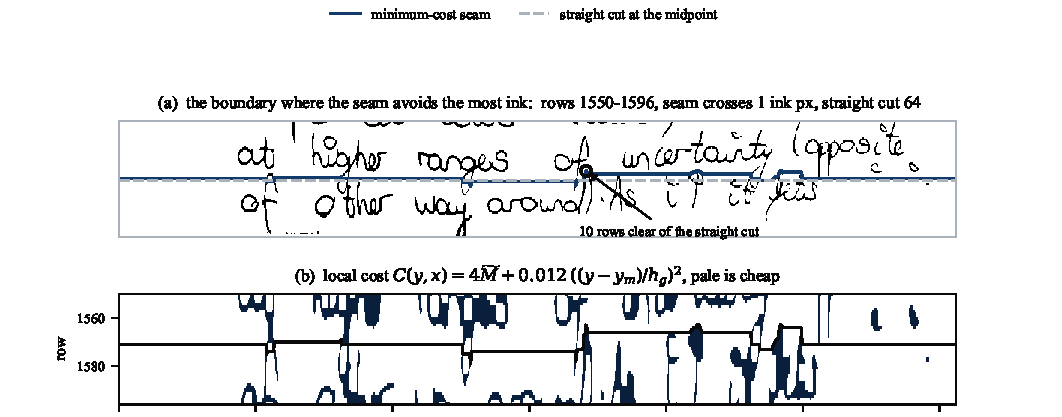
\includegraphics[width=0.96\linewidth]{Figures/design-seam-two-panels.pdf}
\caption{Seam path and its cost field.}
\label{fig:des-seam-example}
\end{figure}

\subsubsection{Assigning ink to the correct line}
A seam divides the page into bands along the calculated boundaries. Dots, ascenders or descenders can still fall into its neighbour's crop. According to research, eight-connected components, found using row runs and union operations, are used to do a check of ownership of extended ink fragments~\cite[pp.~476--479]{rosenfeld1966}.

For each component, a band containing at least 15\% of its in-band ink is considered important. The uppermost substantial band supplies the reference owner for eligible small-piece corrections. If none qualifies, the largest overlap in text features is used. Large collections of text generally keep their ownership of text, except for the narrow-tail and small-piece rules.

For example, an \texttt{i} dot may lie above the seam while its stem supports assignment to the lower line. Raw components are revisited because closing may join the dot to an unrelated stroke. Enclosed-ring and residual-fragment checks handle further detached pieces. Algorithm~\ref{alg:des-ownership} gives this order, with $O$ storing each pixel's line index.
\begin{designalgorithm}
\caption{Refining seam bands into ink ownership}
\label{alg:des-ownership}
\prequire{Ink mask $M$, components $\mathcal C$, seams, centres and pitch $P$.}
\begin{designpseudo}
\pstate{0}{\textbf{for each} component $C\in\mathcal C$ \textbf{do}}
\pstate{1}{Count overlap $a_{C,n}$ with each seam band $n$}
\pstate{1}{$S=\{n:a_{C,n}\geq0.15\sum_j a_{C,j}\}$}
\pstate{1}{Choose topmost $S$ as reference owner, or maximum overlap if S is not 0}
\pstate{1}{Correct eligible narrow tails and small pieces, reject remote little specks}
\pstate{1}{Associate compact dots with plausible stems using pitch-scaled guards}
\pstate{0}{\textbf{end for}}
\pstate{0}{$O=$ corrected ownership, preserving large-piece seam assignments}
\pstate{0}{\textbf{for each} raw component near a neighbouring line \textbf{do}}
\pstate{1}{\textbf{if} detached-dot or enclosed-ring guards pass \textbf{then}}
\pstate{2}{Transfer eligible pixels to the supported stem's line, protect correction}
\pstate{1}{\textbf{end if}}
\pstate{0}{\textbf{end for}}
\pstate{0}{Reassign residual fragments lacking their own body-band support}
\pstate{0}{\textbf{return} $O$, excluded pixels keep no line index}
\end{designpseudo}
\end{designalgorithm}

Figure~\ref{fig:vt-ownership} shows the three largest corrections on an example page written by author A. The boxes mark the affected pieces and colour shows the assigned line. The complete page has 462 reassigned pixels. This count actually shows all the rules in action by the colour of their text, with all text of the same colour belonging to the same crop. The first row shows the line before correction, while the second row corresponds to the after correction according to the rules.
\begin{figure}[H]\centering
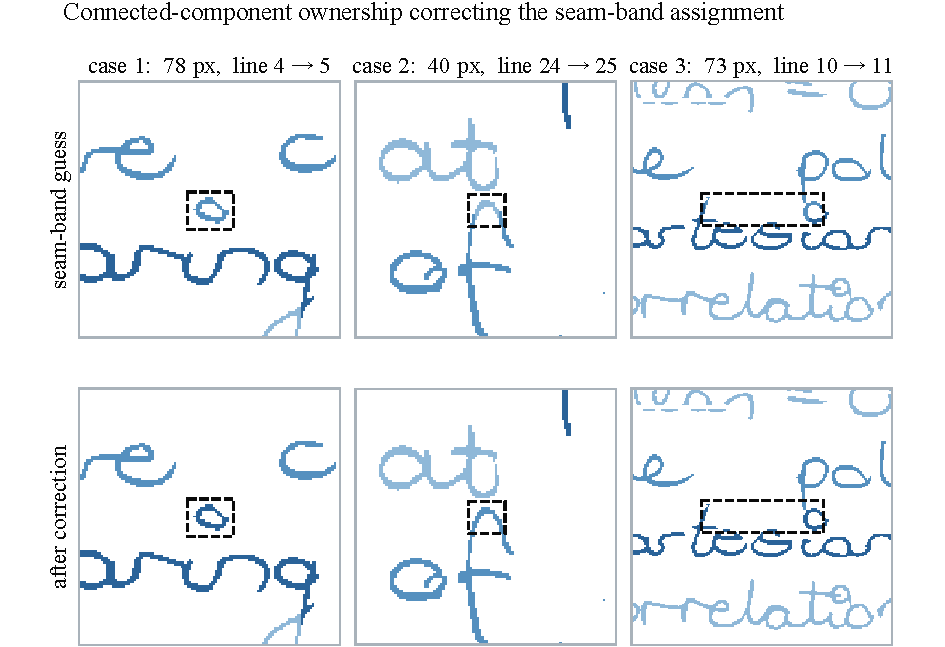
\includegraphics[width=0.96\linewidth]{Figures/VisualTests/T27_ownership_corrections.pdf}
\caption{Ink ownership before and after correction.}
\label{fig:vt-ownership}
\end{figure}

\subsubsection{Preparing the classifier crops}
Crops are constructed from the original resolution picture after ownership is settled. A soft ink mask stays away from jagged edges, while a separate nearest-neighbour ownership exclusion keeps neighbouring ink out. Contrast stretching and a darkness exponent of 0.55 strengthen faint alows strokes to be kept.

A guard in place to ensure better crops reject a line only when its dark-pixel fraction (the number of ink or shadow pixels over the number of pixels in the crop) exceeds both 15\% and is 3 times the amount of the page median. If every crop would be rejected, the input list is kept. The guard therefore is able to reduce solid-shadow crops without actually checking that every remaining crop is stil right.

To prepare the cropped image for the classifier, it must be fitted to the desired input size. The classifier canvas is $64\times640$ pixels. A common scale preserves the proportions of a crop of height $h$ and width $w$, to ensure an image is not stretched, and that its aspect ratio is kept.
\begin{equation}
a=\min\left(\frac{64}{h},\frac{640}{w}\right),\qquad
(h',w')=(ah,aw).
\label{eq:des-fit}
\end{equation}

For the archived $156\times2170$ dataset line, $a\simeq0.295$ gives a $46\times640$ image. It is left-aligned, vertically centred and padded white. A very long line loses vertical detail when the width limit controls this scale. INCLUDE IMAGE

\subsubsection{Complete processing sequence and output}
Figure~\ref{fig:des-seg-stages} follows the page from lighting correction to ink extraction, line boundaries and final crops. These views show where a stroke was removed or assigned to another line. Algorithm~\ref{alg:des-segment} gives the full sequence after the individual operations described above.
\begin{figure}[H]\centering
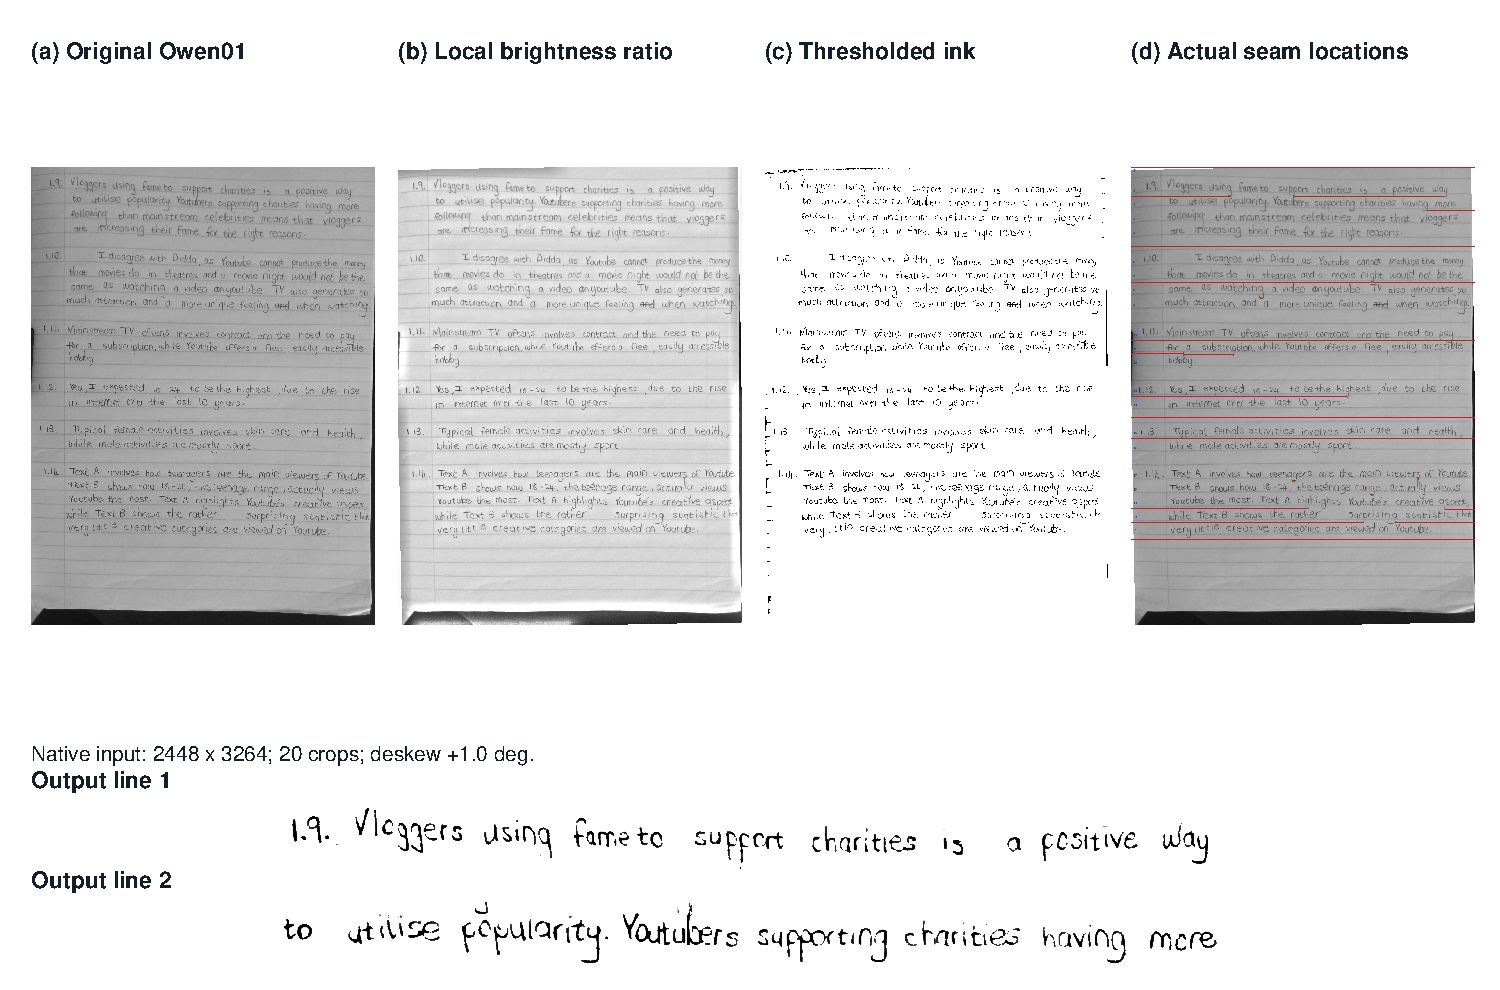
\includegraphics[width=0.96\linewidth]{Figures/design-segmentation-stages.pdf}
\caption{Page preparation and line extraction.}
\label{fig:des-seg-stages}
\end{figure}

In the algorithm, $G_f,G_h$ are the full and half-resolution grey images, $R$ is the brightness ratio and $M$ is the ink mask. Pitch $P$, centres $c$ and seams $b$ define the lines. The output $\mathcal L$ contains the ordered crops, classifier views and bounding boxes.
\begin{designalgorithm}
\caption{Photographed page to ordered line crops}
\label{alg:des-segment}
\prequire{Grey page on its chosen line axis.}
\pensure{Ordered full-resolution crops, coordinates and diagnostics.}
\begin{designpseudo}
\pstate{0}{$(G_f,G_h,M,R,\theta)\leftarrow\operatorname{Deskew}(G)$}
\pstate{0}{$M\leftarrow\operatorname{RemovePrintedStructure}(M,G_h)$}
\pstate{0}{$(M,\mathcal C)\leftarrow\operatorname{DropArtifactPieces}(M,R)$}
\pstate{0}{$(P,c)\leftarrow\operatorname{LineCentres}(M)$}
\pstate{0}{$b\leftarrow\operatorname{SeamCuts}(M,c,P)$}
\pstate{0}{$O\leftarrow\operatorname{AssignOwnership}(M,\mathcal C,b,c,P)$}
\pstate{0}{$\mathcal L\leftarrow\varnothing$; normalise full-resolution brightness}
\pstate{0}{\textbf{for each} line index $n$ \textbf{do}}
\pstate{1}{$C_n\leftarrow\operatorname{BuildLineCrop}(n,O,G_f,P)$}
\pstate{1}{\textbf{if} $C_n$ has sufficient ink and height \textbf{then}}
\pstate{2}{Append $C_n$, its fixed-canvas view and bounding box to $\mathcal L$}
\pstate{1}{\textbf{end if}}
\pstate{0}{\textbf{end for}}
\pstate{0}{$\mathcal L\leftarrow\operatorname{DropSolidCrops}(\mathcal L)$; renumber retained crops}
\pstate{0}{\textbf{return} $\mathcal L$, seams, ratio image and diagnostics}
\end{designpseudo}
\end{designalgorithm}

After cropping, the reader compares up to three sampled lines in both directions to distinguish upright from upside-down writing. It chooses the higher mean frame log score, reuses those readings and reverses line order when needed. This heuristic can still fail when the reader is confidently wrong.

\subsubsection{Segmentation verification and limitations}
\label{sec:des-segverify}
The native Owen01 page produces 20 crops for 20 labelled lines. Figure~\ref{fig:des-seg-variation} tests a harder sparse page photographed three times. The striped-shadow image gives three crops, the diffuse-shadow image four, and the changed-angle image 28. In the last case, gap scores of 0.379 and 0.400 give only a 1.054 ratio, below the 1.35 turn threshold. Fine deskewing cannot repair the missed quarter turn.
\begin{figure}[H]\centering
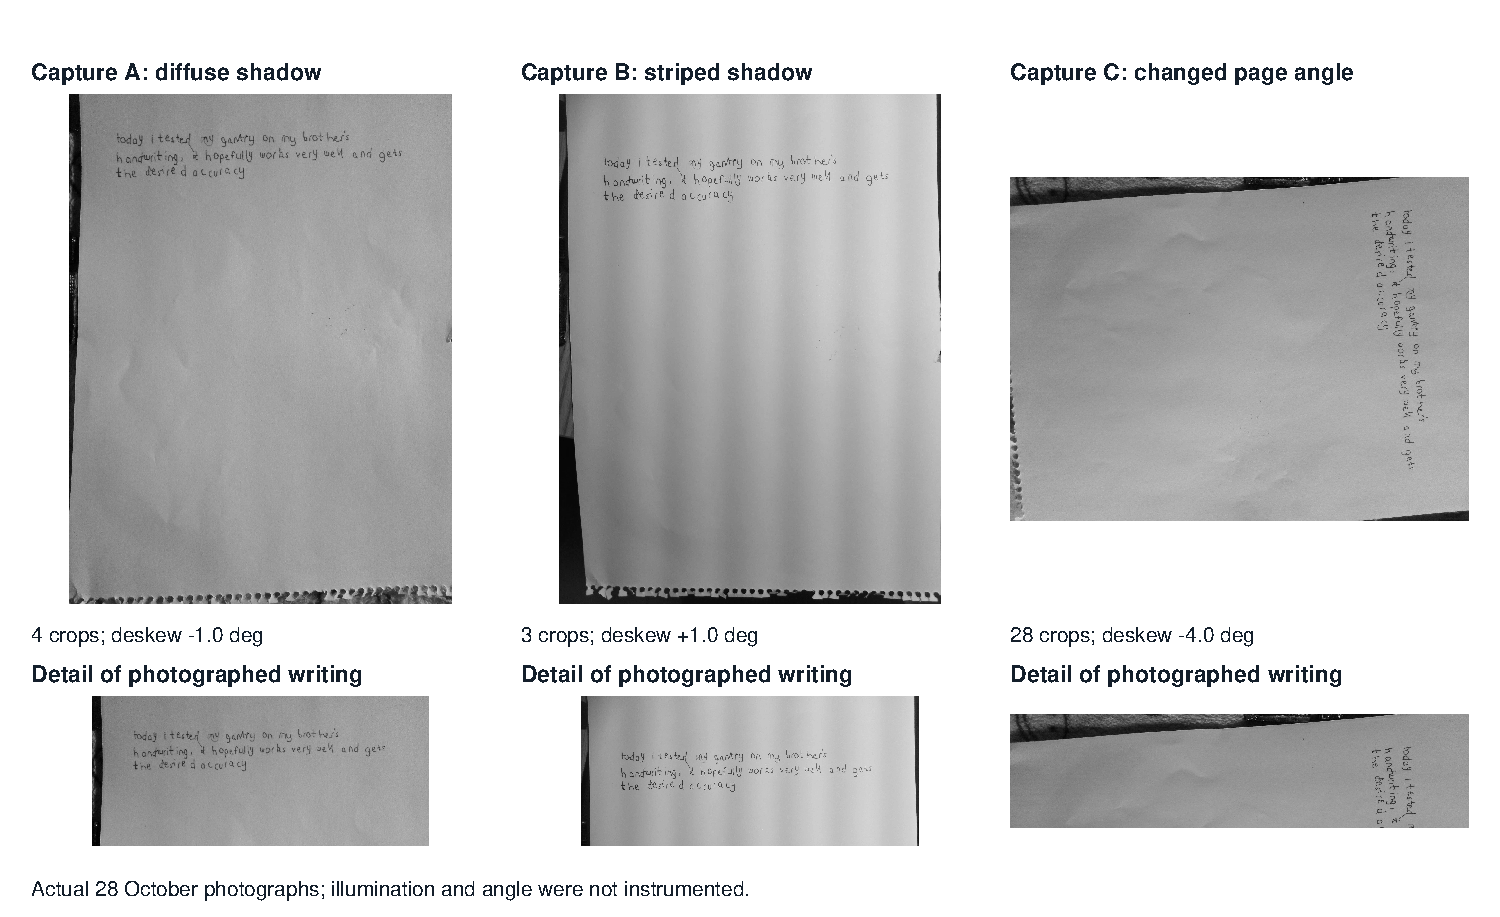
\includegraphics[width=0.95\linewidth]{Figures/design-segmentation-variation.pdf}
\caption{Three captures of the same sparse page.}
\label{fig:des-seg-variation}
\end{figure}

These captures show failure conditions rather than a measured lighting range. Irregular spacing weakens pitch estimation, touching strokes can defeat ownership, and sparse pages provide little orientation evidence. A fixed mount and restrained page reduce perspective and curvature that a global rotation cannot correct. Appendix~\ref{app:des-visual-tests} retains the capture records and extended checks.
\FloatBarrier
